\input{PreambleCommon}
\newcommand{\WeekTitleOne}{Derivatives - Foundations}
\newcommand{\WeekTitleTwo}{Derivatives - Linearization and Applications}
\newcommand{\WeekTitleThree}{Derivatives - Applications}
\newcommand{\WeekTitleFour}{Integrals - Foundations}
\newcommand{\WeekTitleFive}{Integrals - Techniques}
\newcommand{\WeekTitleSix}{Integrals - Modeling}
\newcommand{\WeekTitleSeven}{Differential Equations - }
\newcommand{\WeekTitleEight}{Differential Equations - }
\newcommand{\WeekTitleNine}{Differential Equations - }
\newcommand{\WeekTitleTen}{Linear Algebra - }
\newcommand{\WeekTitleEleven}{Linear Algebra - }
\newcommand{\WeekTitleTwelve}{Linear Algebra - }



\begin{document}
\setfont
\pagestyle{fancy}
\renewcommand{\Week}{6 }
\renewcommand{\WeekTitle}{\WeekTitleSix }

\fancyhead[LE,RO]{Week \Week}  % default, usually only for first page
\fancyfoot{}
\sectionbox{Week \#\Week: \WeekTitle}


\vspace{5mm}
\goals
\begin{itemize}
\item Use MATLAB to solve a variety of integration problems. 
\item Use integration to find the average value of a function.
\item Use MATLAB to find the average value of a function. 
\item Applications of Integration.
\end{itemize}
\vspace{5mm}


\topic{Heat Transfer and Integrals}
\subsection*{Heat Transfer and Integrals}
A common engineering challenge is to transfer heat generated by a
motor or combustion into a nearby fluid.

This transfer is often made more effective by the use of {\bf cooling
  fins}, which increase the surface area of contact with the fluid.

\begin{center}
  \includegraphics[width=5in]{graphics/notes_06_LongPin3D}
\end{center}

If we fix the temperature at the base, we can ask the question \\
{\bf ``How quickly is heat radiated out of fin?''}

\newpage

\problem What factors affect the rate of heat transfer out of the
  fin?

\begin{center}
\includegraphics[width=3.5in]{graphics/notes_06_LongPin3D}
\end{center}

\vfill
\vfill

\newpage

Newton's Law of Heating and Cooling tells us that the rate of heat
flow from a metal fin to the environment is proportional to the
temperature difference between the fin, $T$, and the environment,
$T_\infty$.
\begin{center}
\includegraphics[width=3.5in]{graphics/notes_06_LongPin3D}
\end{center}

\problem What issue is raised when trying to use this rule to compute
the rate of heat flow out of the fin we are considering?
 

\newpage
\topic{Numerical Integration - Motivation}
\subsection*{Numerical Integration - Motivation}

\problem Take a small slice of length $\Delta x$ of the fin.  What
advantage is there to looking at a small slice, rather than the whole
fin at once?
\vfill

How much heat is lost through that slice?
\begin{center}
\includegraphics[width=3.5in]{graphics/notes_06_LongPin3D}
\end{center}

\vfill

Give an expression for the total amount of heat lost over
  the whole fin.

\vfill
\vfill


\newpage


\subsection*{Integration}

As soon as you see any sum of the form $\sum \ldots \Delta x$, you
should be thinking ``integral''!

\problem For our fin example, net heat flow to environment is given
by:
%\begin{align*}
%\int_S h (T(x) - T_{\infty} )~dA 
%\end{align*}
\vfill
If, for simplicity, we assume $T_{\infty} = 0$, our target integral becomes:
%\begin{align*}
%\mbox{Heat rate} = \int_S h ~T(x)~dA 
%\end{align*}
\vfill

\newpage

\subsection*{Finding the Temperature Distribution}
To evaluate the integral, we first need to find the temperature
distribution along the fin.  Without getting into all the gory
details, tables or other methods will lead to the following formula
for the temperature along the fin:

$$T(x) = \frac{T_b \left(\cosh(m(L-x)) + \frac{h}{mk}\right)\left(\sinh(m(L-x))\right)}{\cosh(mL) + \frac{h}{mk} \sinh(mL)}, m = \sqrt{\frac{hP}{k A_c}}$$

\problem What are these new $\cosh(x)$ and $\sinh(x)$ functions?
\vfill

What does the $m$ parameter capture in the physics of the scenario?
\vfill



\newpage
\subsection*{Graphically}
Once we have the temperature distribution, we can graph it along the
length of the fin to see if it makes sense.

\begin{center}
\begin{minipage}{4.0in}
\includegraphics[width=4.0in]{graphics/notes_06_LongPin3D}
\end{minipage}
\begin{minipage}{4.0in}
\begin{center}
\includegraphics[height=4.0in]{graphics/notes_06_FinTemperature1}
\end{center}
\end{minipage}
\end{center}
\newpage

\begin{center}
\begin{minipage}{4.0in}
\includegraphics[width=4.0in]{graphics/notes_06_LongPin3D}
\end{minipage}
\begin{minipage}{4.0in}
\begin{center}
\includegraphics[height=4.0in]{graphics/notes_06_FinTemperature1}
\end{center}
\end{minipage}
\end{center}

Our next step is to see if we can use this temperature distribution,
$T(x)$, to compute the rate of heat transfer by integration:
$$
Q = \int_0^{L} h ~P ~T(x) ~dx   ~~~~~~~~~~ (T_\infty \mbox{ assumed = 0})
$$


\newpage


\topic{Computing Total Heat Loss}
\subsection*{Computing Total Heat Loss}
Now, we have addressed one challenge in our problem: we know the
steady-state temperature along the fin.  Next, we want to compute
the net rate of heat flow out, or the cooling ability of the fin.

The heat flow out of the fin is given by
$$
Q = \int_0^{L} h ~P ~T(x) ~dx   ~~~~~~~~~~ (T_\infty \mbox{ assumed = 0})
$$
Our first approach, if it is possible, should be direct
anti-differentiation (think $\int x^2 ~dx = \frac{1}{3}x^3$).

\newpage
$$
Q = \int_0^{L} h ~P ~T(x) ~dx   ~~~~~~~~~~ (T_\infty \mbox{ assumed = 0})
$$

For this problem, given the earlier temperature we found, $T(x)$, we
{\bf can} evaluate the integral exactly: \\[1ex]
$$ \large
Q =
\frac{1}{2}\frac{T_b~P~h~(m~k~exp(2~m~L)-m~k+h~exp(2~m~L)+h-2~h~exp(m~L))}{m(\cosh(m~L)~m~k+h~\sinh(m~L))~exp(-m~L)}
$$ 

Evaluated with appropriate constants for the material, base temp,
etc. we would obtain the final value $$Q = 2.363 \mbox{ J/s}$$

\begin{center}
\includegraphics[width=3.5in]{graphics/notes_06_LongPin3D}
\end{center}
\newpage

\subsection*{Comments on Anti-Derivatives}

Through this last step, we reached what would be the important
engineering goal: obtaining the {\bf numerical value} for the
integral.

When we compute integrals analytically, by using anti-derivatives, we
are doing the best possible thing. 
\begin{itemize}
\item Integrals give exact values.
\item Integrals can be re-used immediately with different constants.
\end{itemize}
Unfortunately, actually computing the numerical value of an integral
using antiderivatives isn't always an option:
\begin{itemize}
\item Some functions don't have antiderivatives.  
\vspace{1cm}
\item Sometimes we don't have a function, but only data.
\vspace{1cm}
\item Sometimes we forget how to find the anti-derivative!
\vspace{1cm}
\end{itemize}

\newpage

\topic{Numerical Quadrature}
\subsection*{Numerical Quadrature}

The word {\em quadrature} comes from the Greek challenge of trying to
{\em square the circle}, or finding the {\bf area} (in square units)
of the round circle.

When you hear {\bf quadrature} think {\bf numerical integration}.

The two common scenarios where we need {\em numerical} integration will be:
\begin{itemize}
\item {\bf Formula} for $f(x)$ known, want $\ds \int_a^b f(x) dx$
\item {\bf Data} for $f(x)$ collected at $f(x_i)$, want $\ds \int_a^b f(x)
  dx$
\end{itemize}
We will study the formula case initially, because it is easier to
experiment with.  We will continue to use our cooling fin example,
where
$$
Q = \int_0^{L} h ~P ~T(x) ~dx = 2.36269950112023 \mbox{ J/s}
$$

\newpage

Graphically, $\displaystyle Q = \int_0^L \underbrace{h~P~T(x)}_{f(x)}~dx$
is the area shown below:
\begin{center}
\includegraphics[height=5cm]{graphics/notes_06_f_graph_with_area}
\end{center}
Numerical integration is performed by:
\begin{itemize}
\item separating the desired interval into {\em panels}, and then
\item on each {\em panel}, evaluating the integrand, $f(x)$ one or
  more times and those values are combined in some way to {\em estimate}
  the area of the panel.
\end{itemize}

\newpage

\subsection*{Left-Hand Sum}
The simplest quadrature rule is one we have already seen: the LEFT($n$) sum.
\begin{itemize}
\item Divide the interval into $n$ panels, width $\Delta x = (b-a) / n$
\item Evaluate the function at the left end point, $f(x_{i-1})$, on
  each panel.
\item Compute the area of rectangles, $\ds \sum_{i=1}^N f(x_{i-1}) \cdot \Delta x$ or
\end{itemize}
\begin{center}
\includegraphics[height=7cm]{graphics/notes_06_f_left_hand_rule}
\end{center}

\newpage

\subsection*{Quadrature Principles}
We are approximating a complex shape with simpler shapes for which we
can compute the area. The {\bf more panels} we use, the {\bf more
  accurate} the area estimate will be:
\begin{center}
\includegraphics[height=6cm]{graphics/notes_06_f_lhr_5_intervals}
\includegraphics[height=6cm]{graphics/notes_06_f_lhr_50_intervals}
\includegraphics[height=6cm]{graphics/notes_06_f_lhr_500_intervals}
\end{center}
By using enough panels, we can reduce the error to any level we like,
but with the trade-off that it takes longer to compute.

\newpage

\problem Download the file
\href{http://www.mast.queensu.ca/~apsc171/MNTCP01/Notes/MATLAB/week06CoolingFin.m}{week06CoolingFin.m},
and extend it so it plots the graph of the temperature along the fin.

Using MATLAB, estimate the integral $\ds Q = \int_0^L h P ~T(x) ~dx$
with the left-hand rule,
$$ Q \approx \sum_{i=1}^n h P ~T(x_{i-1})~ \Delta x$$

\vsc

\newpage

\problem Add a statement that displays the number of intervals used,
$n$, and the resulting error in the LEFT($n$) integral estimate. \\
Experiment by doubling the number of intervals and seeing the
resultant reduction in error.

\vsc

When you double the number of intervals, what happens to the error?

\vfill

Note: If you are using computer software for modeling in your career,
it would be a good idea to get familiar with {\em numerical methods}
and {\em numerical analysis} concepts.

\newpage 
\topic{Built-In Integration in MATLAB }
\subsection*{Built-In Integration in MATLAB }

Previously, we have used the LEFT($n$) approximation to estimate the
value of an integral, both by hand and using MATLAB to speed up the
computation.

As you might expect, numerical integration is something we can do
using built-in MATLAB functions, instead of writing our own LEFT($n$)
rule.

\problem Look up the functions \texttt{quad} and \texttt{integral} in
MATLAB help.

\vsc

\newpage

\problem Starting with
\href{http://www.mast.queensu.ca/~apsc171/MNTCP01/Notes/MATLAB/week06CoolingFin.m}{week06CoolingFin.m},
use \texttt{quad} or \texttt{integral} to evaluate the rate of heat
transfer from the cooling fin.  Compare it with the exact integral
value,

$$
Q = \int_0^{L} h ~P ~T(x) ~dx = 2.36269950112023 \mbox{ J/s}
$$


Experiment with additional options that could be used to increase the
accuracy of the numerical integral estimate.


\newpage

\topic{Numerical Integration in MATLAB - Examples}
\subsection*{Numerical Integration in MATLAB - Examples}

We now have two techniques we can try when evaluating definite
integrals like $\ds \int_a^b f(x)~dx$ where the formula for $f(x)$ is
given:
\begin{itemize}
\item The Fundamental Theorem of Calculus: finding an anti-derivative
  $F(x)$ then evaluating $F(b) - F(a)$;  or \\[1ex]
\item Numerical integration tools. \\[1ex]
\end{itemize}

\newpage

\problem Use the Fundamental Theorem of Calculus to evaluate the
integral
$$\int_1^3 \ln(x)~dx.$$

\vfill

Use the built-in numerical integration tools in MATLAB to estimate the
value of
$$\int_1^3 \ln(x)~dx.$$
\vspace{1in}


\newpage
\problem Use the Fundamental Theorem of Calculus to evaluate the
integral
$$\int_0^{\pi} x^2 \cos(x^3)~dx.$$

\vfill

Use the built-in numerical integration tools in MATLAB to estimate the
value of
$$\int_0^{\pi} x^2 \cos(x^3)~dx.$$
\vspace{1in}

\newpage
\problem Try to use the Fundamental Theorem of Calculus to evaluate
the integral
$$\int_{-2}^{2} e^{-x^2}~dx.$$

\vfill

\newpage

\problem Use MATLAB to plot the graph of $f(x) = e^{-x^2}$ on the
interval $x\in [-2, 2]$.

\vspace{1in}

Sketch the graphical interpretation of the integral
$$\int_{-2}^{2} e^{-x^2}~dx.$$
\vfill

Use the built-in numerical integration tools in MATLAB to estimate the
value of
$$\int_{-2}^{2} e^{-x^2}~dx.$$
\vspace{1in}

\newpage

\topic{Applications of Integrals - Average Value}
\section*{Applications of Integrals - Average Value}

\problem If the following graph describes the level of $CO_2$ in the
  air in a mine over a week, estimate the {\em average level} of
  $CO_2$ over that period.

\hfill 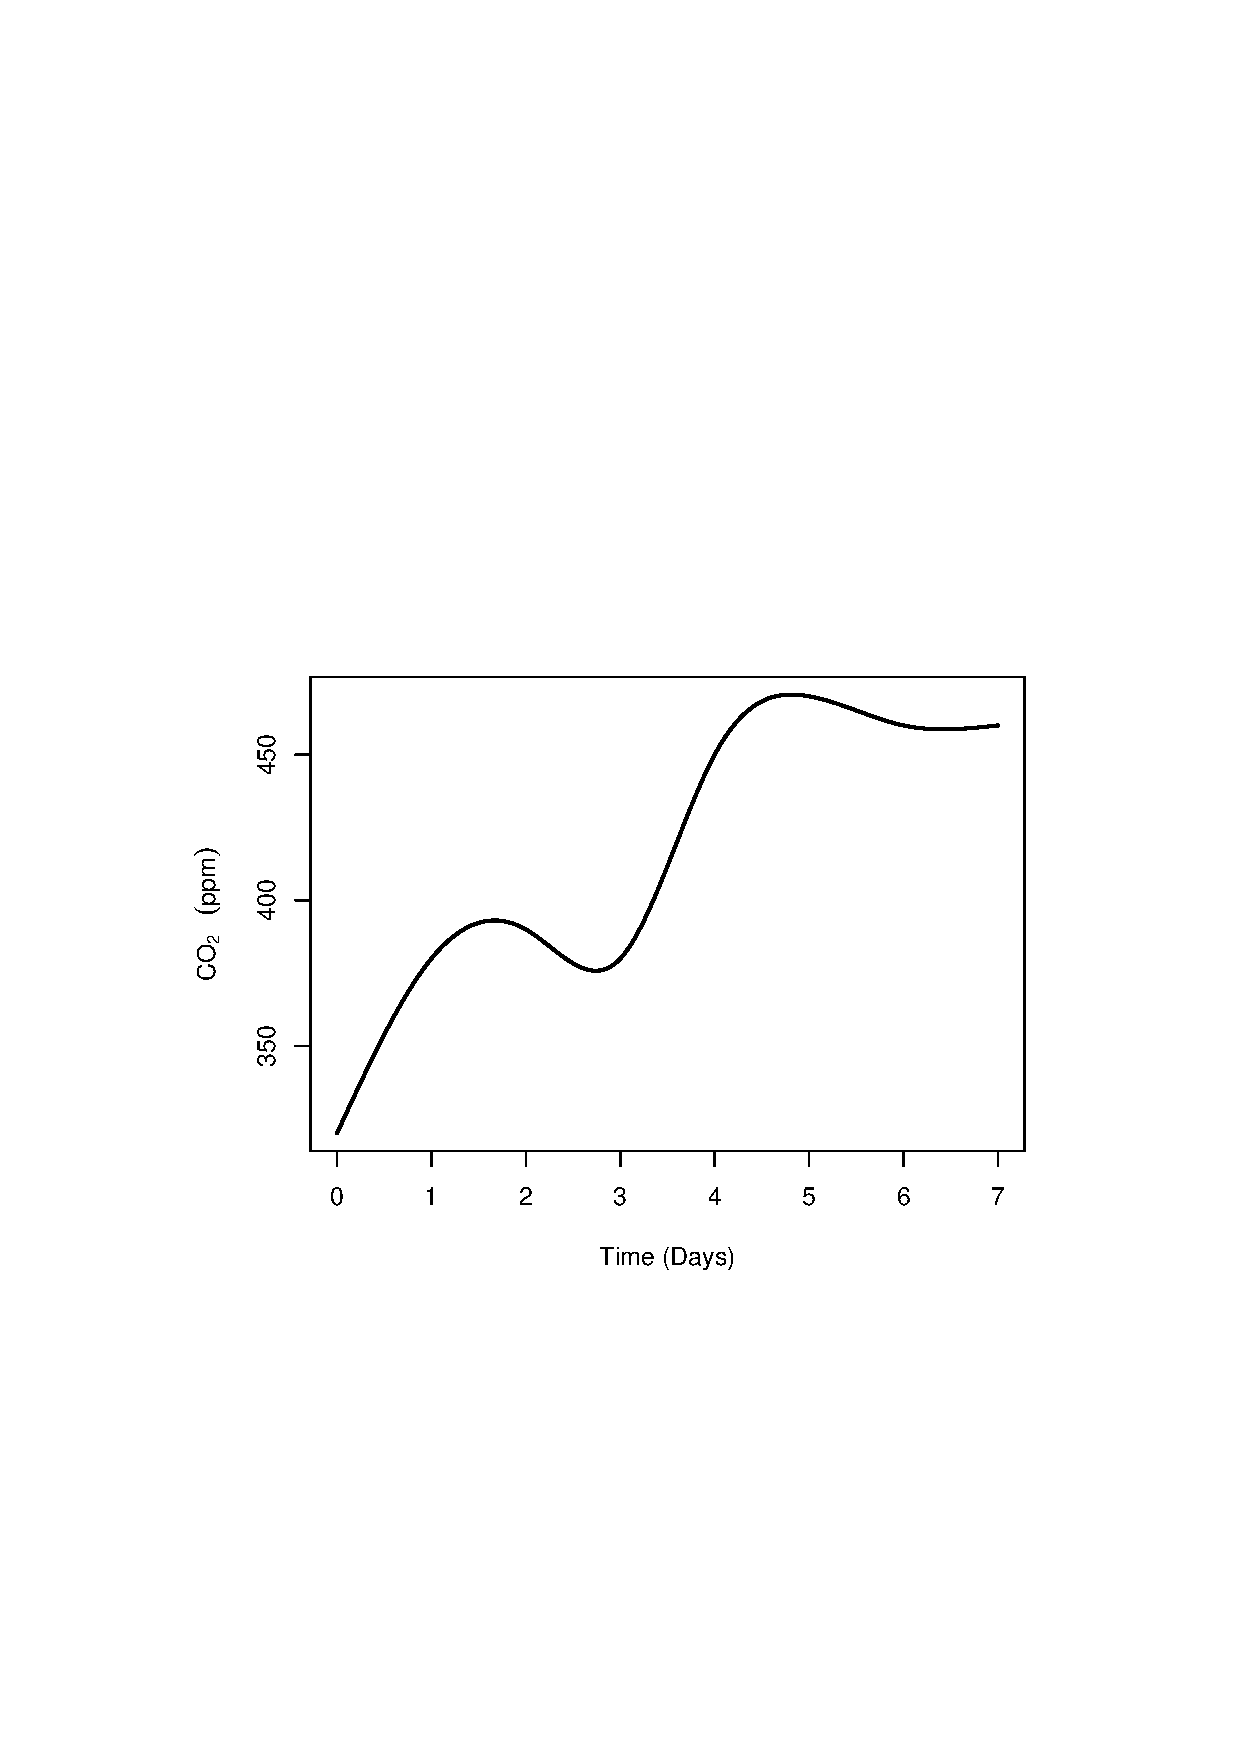
\includegraphics[width=3.8in]{graphics/notes_06_graph02}

\problem Give the units of the average $CO_2$ level.

\vspace{1in}

\newpage

\problem Sketch the graph of $f(x) = x^2$ from $x=-2$ to $2$, and
  estimate the average value of $f$ on that interval.

\hfill \includegraphics[width=3in]{graphics/empty_graph_square_8}

\newpage

\problem What makes the single ``average'' $f$ value different or
  distinct from other possible $f$ values?


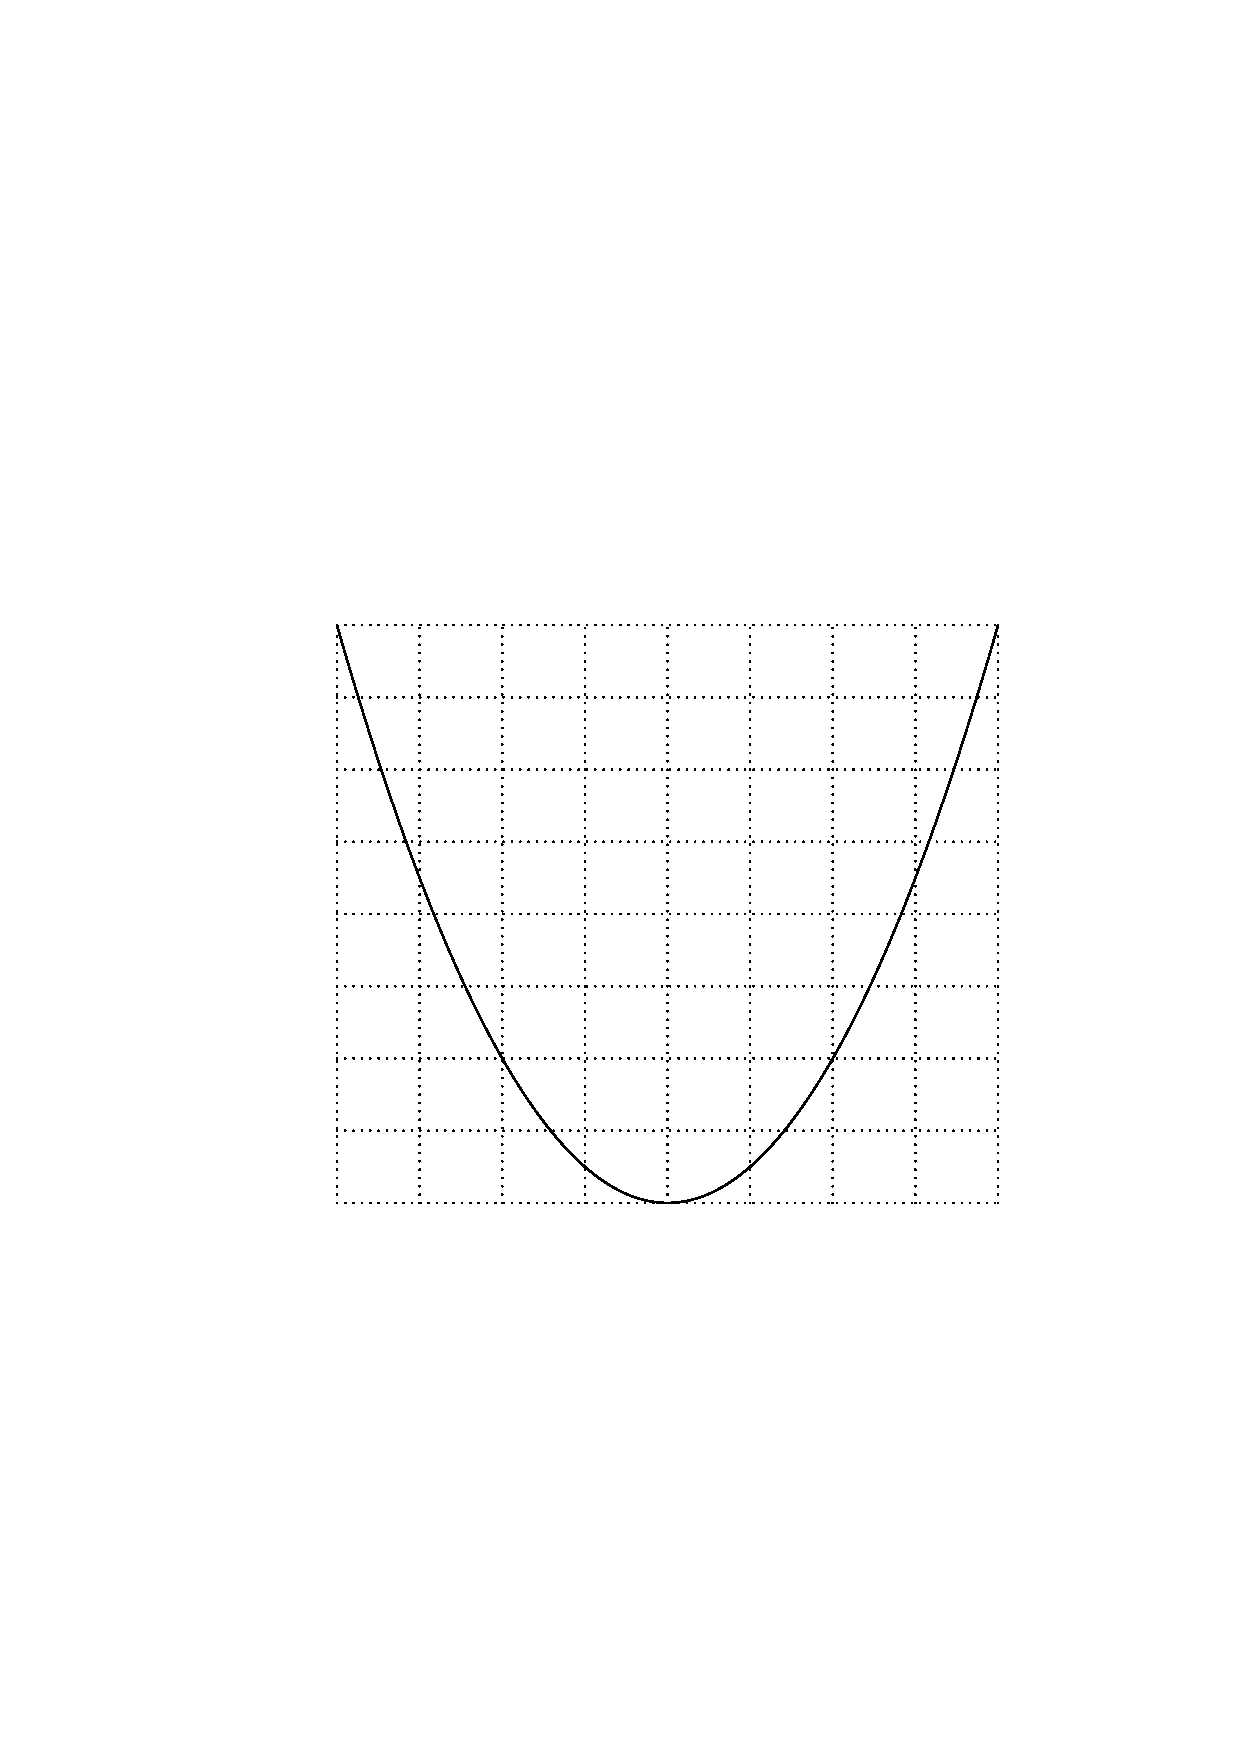
\includegraphics[width=3in]{graphics/notes_06_quadratic}\hfill
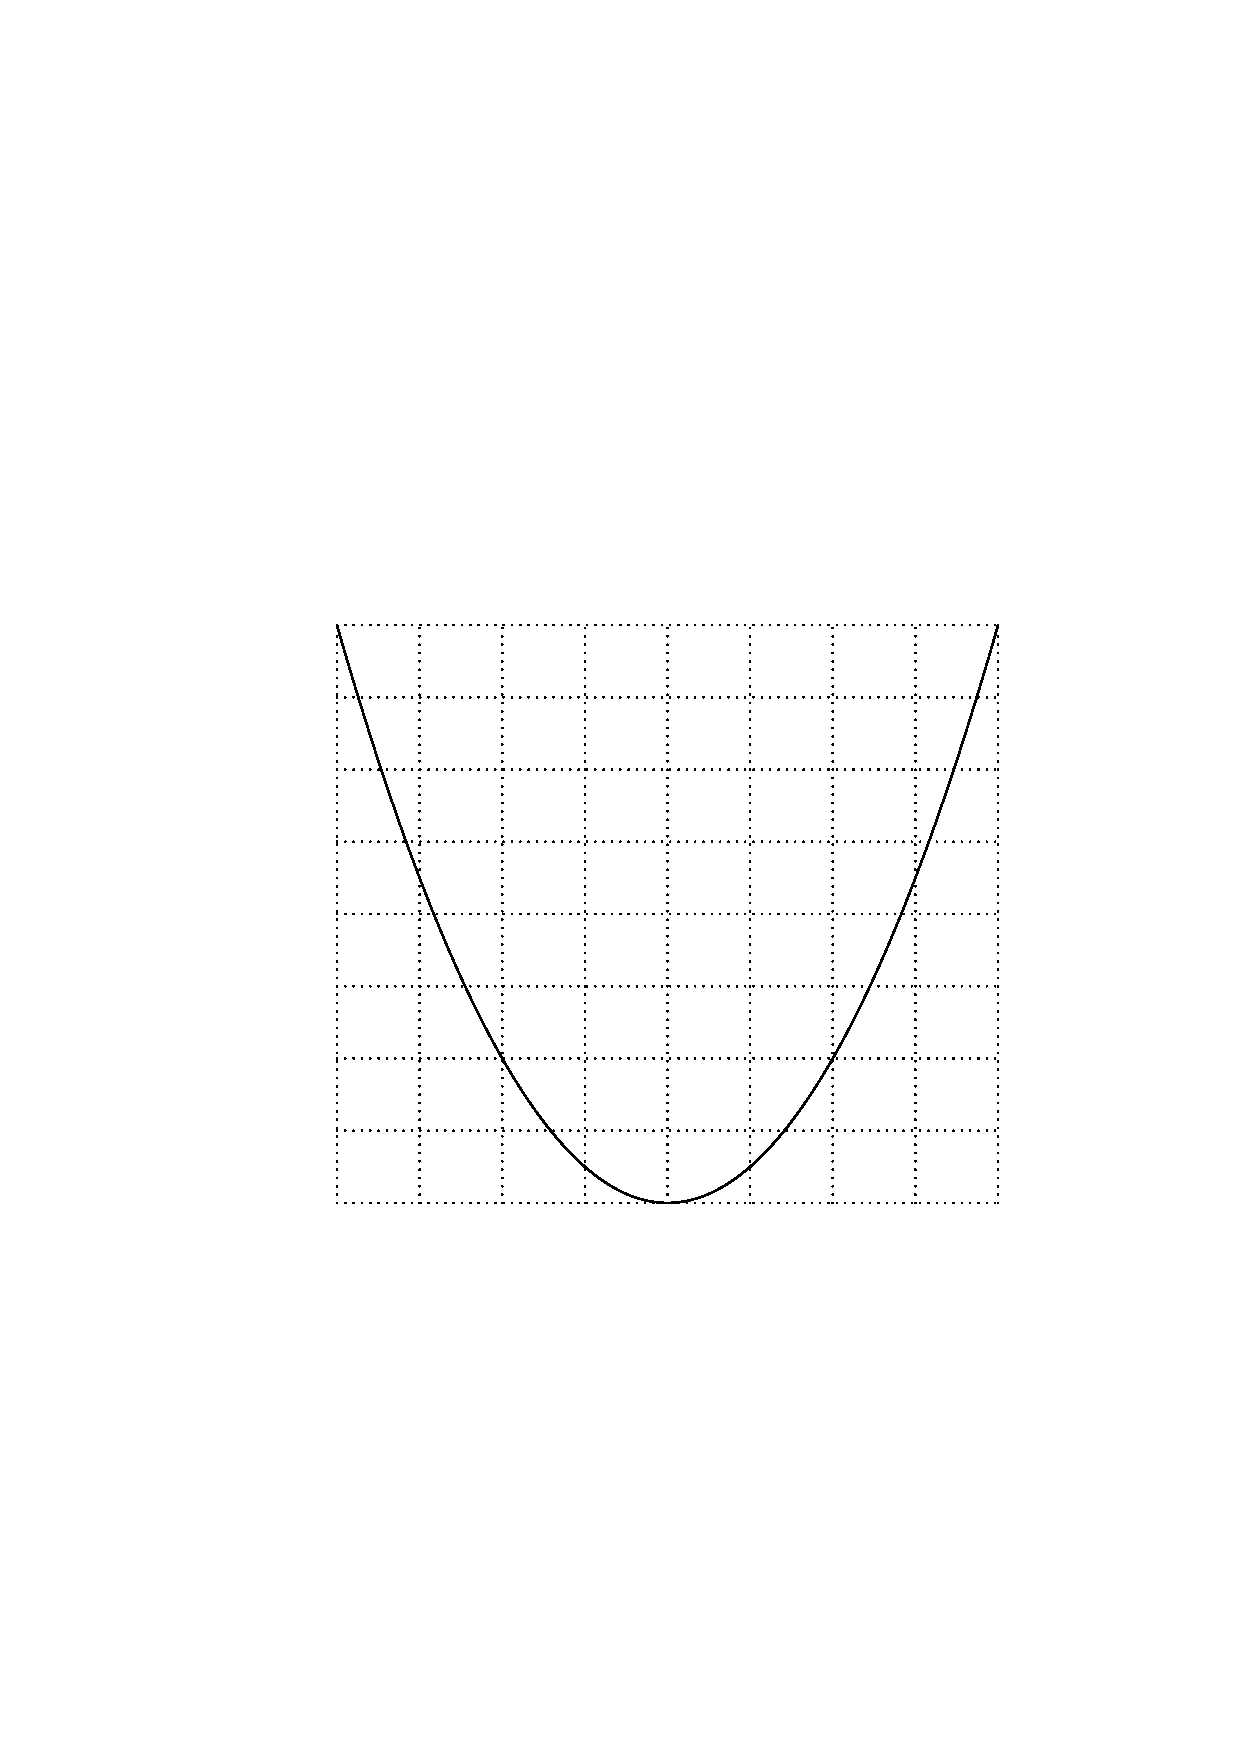
\includegraphics[width=3in]{graphics/notes_06_quadratic}\hfill
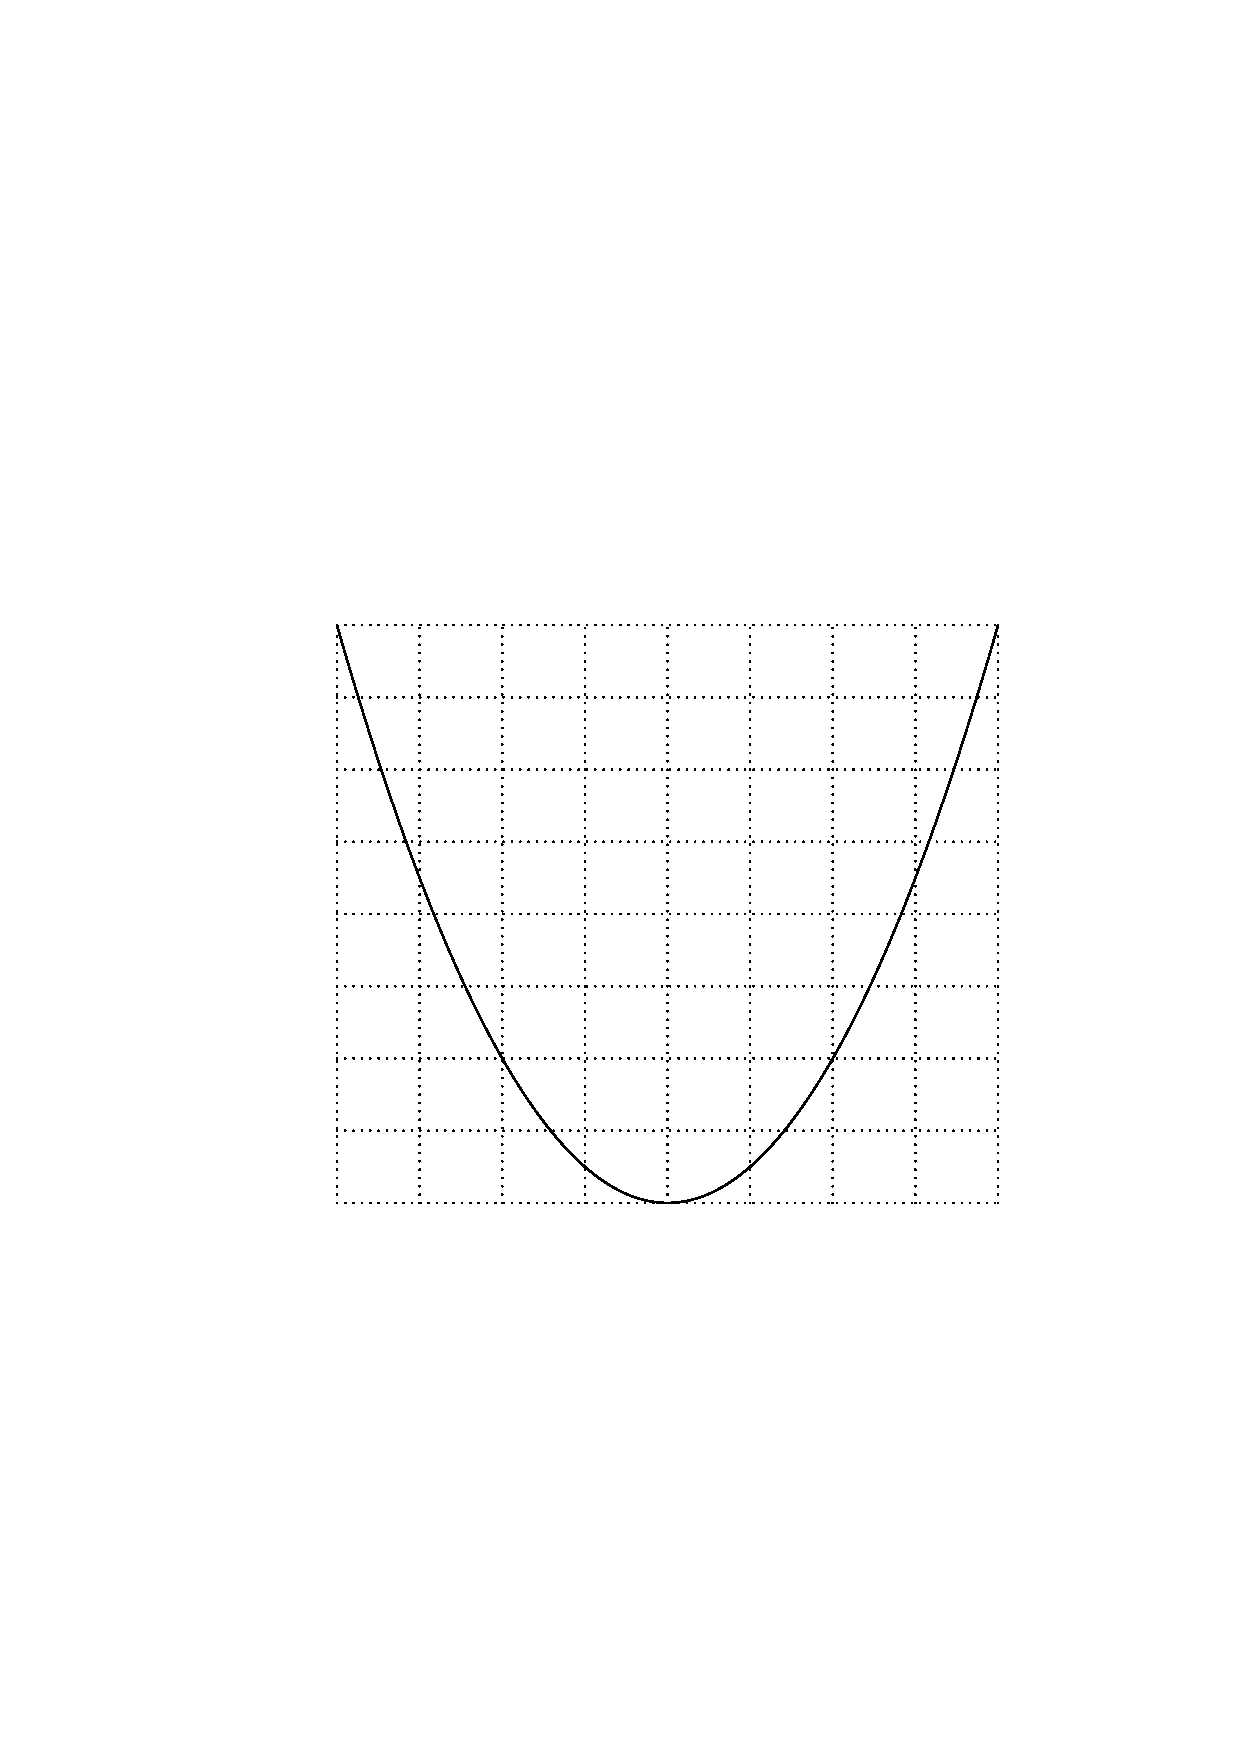
\includegraphics[width=3in]{graphics/notes_06_quadratic}

\problem Use this property to find a general expression for the
  {\bf average value of $f(x)$ on the interval $x \in [a, b]$}.

\vfill

\newpage

\problem Find the exact average of $f(x) = x^2$ on the interval $x \in
  [-2, 2]$ using this formula.

\vfill

\newpage 
\problem Use MATLAB to generate a graph of $f(x) = x^2$, compute the
average value using the built-in integration tools, and then add a
line at the average value.  Use the same $x \in [-2, 2]$ interval.

\newpage

\topic{Average Value - Temperature Example}

\begin{boxnote}
  {\bf Average Value of a Function on $[a, b]$} \\
The average value of a function $f(x)$ on the interval $[a, b]$ is given by 
\begin{align*}
A = \frac{1}{b-a} \int_a^b f(x)~dx 
\end{align*}
\end{boxnote}


\newpage

The temperature in a house is given by $$H(t) = 18 + 4
  \sin(\pi t/12),$$ where $t$ is in hours and $H$ is degrees C.  

  \problem Sketch the graph of $H(t)$ from $t=0$ to $t=12$, then find
  the average temperature between $t=0$ and $t=12$.

\hfill \includegraphics[width=4in]{graphics/empty_graph_wide_12}

\vfill
\vfill

\newpage 
\problem Repeat your analysis for the temperature function
$$H(t) = 18 + 4 \sin(\pi t/12)$$ in MATLAB.  

Include a graph of $H(t)$ over $t = 0\ldots 12$ and a line showing the
average value.

\newpage

\topic{Average Value from Data}
\subsection*{Average Value from Data}

One of the major consumers of electricity in a mining operation is
running the crushers.  Being able to track the efficiency and power
demand of these machines is therefore an important component of
managing mine operations.

Sensors can record the power draw (in MW) over time, and record them
to a spreadsheet.

\problem Download the file
\href{http://www.mast.queensu.ca/~apsc171/MNTCP01/Notes/MATLAB/week06CrusherData.csv}{week06CrusherData.csv}
and either open it in Excel, or double-click on it in the MATLAB File
Viewer.  \vfill

The data in this file contains data for one 24 hour period, in 2 columns:
\begin{itemize}
\item Time (in hours after midnight), and
\item Power (in MW) for the crusher. 
\end{itemize}

\newpage

MATLAB can import Comma Separated Variable (CSV) files easily, though
it does require some new-to-us tools for manipulating matrices.

\problem Explain what each line in this MATLAB script does, and what each variable
will contain.
\begin{verbatim}
M = csvread('week06CrusherData.csv')


t = M(:, 1);


P = M(:, 2);


plot(t, P);
\end{verbatim}

\newpage

\problem How would the total power consumption over the day be
represented mathematically, if $t$ is in hours and $P(t)$ represented
the power being used at hour $t$?

\vfill

Can we compute this value using the Fundamental Theorem of Calculus?

\vfill

\newpage

\problem Write out the Riemann sum approximation to the integral.

\vfill
\vfill

Use MATLAB to estimate the total power consumed during the 24 recorded
hours.
\newpage

\problem Use our earlier formula for average values to estimate the
{\bf average} power consumption rate over 24 hours.

\vfill

Given the data format in MATLAB, find the average power consumption
rate in a different (more traditional) way.

\vfill

Plot both the power consumption over time, and the average power usage
graphically.  \vspace{1in}

\newpage

\topic{Integration and Averages from Data - Acceleration}
\subsection*{Integration and Averages from Data - Acceleration}

Accelerometers are now relatively inexpensive sensors that can be
incorporated in machinery and can be used to infer changes in velocity
and changes in position.

In testing a new collection accelerometer sensors, you attach them to
a cart and record the acceleration over a 6 minute test interval,
running the cart at several different motor powers as the cart moves
from a minehead to a dropoff area.  The cart starts at rest, and is
stopped (zero velocity) before the end of the recording.

The acceleration data is recorded in the file 
\href{http://www.mast.queensu.ca/~apsc171/MNTCP01/Notes/MATLAB/week06CartAcceleration.csv}{week06CartAcceleration.csv}

\newpage

\problem In MATLAB, load the data from
\href{http://www.mast.queensu.ca/~apsc171/MNTCP01/Notes/MATLAB/week06CartAcceleration.csv}{week06CartAcceleration.csv}
and plot the acceleration against time graph.  \\
Time is recorded in seconds, and acceleration in m/s$^2$. \\
Add a black line at $a = 0$ so you can see forwards vs backwards
accelerations more easily.

\vspace{1in} 

Describe in words what the motion of the cart would have looked like,
based just on the acceleration records.

\vfill

\newpage

\problem Write an integral that represents the total change in
velocity for the cart over the six minutes.

\vfill

Can we compute this value using the Fundamental Theorem of Calculus?

\vfill

\newpage

\problem Write out the Riemann sum approximation to the integral that
computes the change in velocity.

\vfill

Use MATLAB to estimate the total change in velocity during the
recording hours.

\vspace{1in}

Comment on the accuracy of the sensors.
\vfill
\vfill

\newpage

\problem Use our earlier formula for average values to estimate the
{\bf average} acceleration over the recording time.

\vspace{1in}

Based on the scenario that was given, should this value be zero as
like the net change in velocity?  Why or why not?

\vfill





















\end{document}

